\chapter{Computer music}

\section{Historical framework}\label{historical-framework}

First experiments in sound synthesis belong to the analogue era.

In the 1950s the study of the Cologne Radio (WDR) was in contrast to the GRM both in:

\begin{itemize}
\tightlist
\item terms of sound generation and manipulation techniques. 
\item terms of aesthetic positions.
\end{itemize}

The reference figure in this study was the composer Karheinz Stockhausen.

At that time his compositional ideas brought the strict rules of serialism into the sound synthesis.

Every parameter of sound (pitch, spectrum, intensity, envelope, duration, etc.) was governed by rigid numerical rules.

The electroacoustic instruments available in the Cologne studio (oscillators, filters and ring modulators) and the possibility of recording the resulting sound on magnetic tape were the ideal tools for developing these ideas.

Karlheinz Stockhausen - \href{http://www.musicaecodice.it/gitmedia/emc/4_media/studio2.mp3}{Elektronische Studie II} for tape (1954) - extract.

Still in the electroacoustic field a mix of the technical equipment of the two studios was found in the RAI Musical Phonology Studio in Milan where the composers of reference were Luciano Berio, Bruno Maderna and later Luigi Nono.

Their aesthetic positions were also less rigid than those of their French and German colleagues, mixing together different compositional techniques.

Bruno Maderna - \href{http://www.musicaecodice.it/gitmedia/emc/4_media/maderna.mp3}{Musica su due dimensioni} for flute and tape (1958) - extract.

Computer music was born later for reasons obviously linked to the birth and development of digital technologies but it takes its cue from these (and other) electroacoustic experiences.

The first computer used for playing music was the CSIR Mk1 developed in Sydney in the late 1940s and presented at a public concert in 1951 where
it performed \href{http://www.musicaecodice.it/gitmedia/emc/4_media/colonel.mp3}{Colonel Bogey March}.

Alan Turing was also working on primeval computer music in the summer of 1951 at the Computing Machine Laboratory in Manchester.

He and his collaborators produced three short \href{http://www.musicaecodice.it/gitmedia/emc/4_media/godsave.mp3}{melodic sequences} played by the computer.

In the late 1950s Max Mathews was the most important computer scientist working at Bell Telephone Laboratories in New Jersey.

He worked primarily with mainframe computers made by IBM on several series of their MUSIC X program, a musical programming language that was upgraded over the next twenty years.

An early piece created in these studios was \href{http://www.musicaecodice.it/gitmedia/emc/4_media/canon.mp3}{Beat Canon} (1960) by J.R.Pierce (director of studio).

In 1963 a \href{http://www.musicaecodice.it/gitmedia/emc/4_media/speech.mp3}{human voice} was synthesized for the first time (speech synthesis).

Later musicians and engineers alike began to collaborate more on the making of music with computers creating more sophisticated work.

Aa example an exrept from \href{http://www.musicaecodice.it/gitmedia/emc/4_media/violin.mp3}{Lyric Variations} for Violin and Computer (1965-1968) by J.K.Randall - extract.

In USA starting from the 60s artistic currents began to develop linked to the Studios and cultural environment where they arose.

\begin{itemize}
\tightlist
\item west coast \(\rightarrow\) \textit{Experimantal Music Studio MIT Media
  Laboratory} - Boston.

  Founded by Barry Vercoe in 1971, it develops software derived from the Music IV series on IBM 360 computers.

  In this studio Curtis Road created Computer Music Journal the world's leading computer music magazine.

  Composers such as James Dashow, Miller Puckette, Charles Dodge worked there, whose approach to composition was characterised by a strong structural rigor derived from the ideas developed by Stockhousen in Cologne.

  Three exemples:

  \begin{itemize}
  \tightlist
  \item James Dashow - \href{http://www.musicaecodice.it/gitmedia/emc/4_media/dashow.mp3}{Conditional Assemblies} for computer generated sounds (1980)
  \item Charles Dodge - \href{http://www.musicaecodice.it/gitmedia/emc/4_media/dodge.mp3}{The Waves} for voice and electronics (1984)
  \item Curtis Road - \href{http://www.musicaecodice.it/gitmedia/emc/4_media/roads.mp3}{Granule} for computer generated sounds (1999)
  \end{itemize}
  
\item california two main poles:

  \begin{itemize}
  \tightlist
  \item Stanford University CCRMA (Karma) \(\rightarrow\) music production.
  \item San Diego University (CARU) and Lucas film studios \(\rightarrow\) software and hardware research.
  \end{itemize}

  The CCRMA was founded and directed by John Chowning, the inventor of FM synthesis and a leading figure in computer music.

  A figure of synthesis between technology and music, he addressed in each of his compositions a specific problem linked both to the synthesis of sound and to musical language.

  Through his work, which also took place in important European production centers such as IRCAM in Paris, he created a bridge between the two continents.

  An \href{http://www.musicaecodice.it/gitmedia/emc/4_media/turenas.mp3}{audio extract} from his work Turenas for computer generated sounds (1972) and a \href{http://www.musicaecodice.it/gitmedia/emc/4_media/turenas.pdf}{paper} about it.
\end{itemize}

\href{https://smcnetwork.org/centers.html}{Here} we can find a comprehensive list of computer music research and production centers.

\section{Randomness}\label{randomness}

Following or pursuing an random procedure means generating or transforming musical or acoustic material by integrating random choices into the decision-making process.

The concept of indeterminism affirms the denial of any determination of the will by external motives.

In our case a sequence of sonic events must be governed in whole or in part by chance or by a set of probabilities, regardless of the author's experience, taste, knowledge, and personality.

This makes it inevitable to rethink the composer's role in the creative act.

A reflection of this kind plays an important role in the poetics of American composer J. Cage who has often stated that his compositional principle is a departure from unity and a movement toward multiplicity:

\textit{ {[}\ldots{]} to abdicate one's subjectivity, to abandon one's own judgment to move toward the multiplicity that is life itself, of which man is but a small component, in the sea of constant variation
{[}\ldots{]}}

In Western musical tradition three different indeterministic procedures have been theorized and used.


\subsection{Chance }\label{chance}

The musical or sonic materials of the piece are:

\begin{itemize}
\tightlist
\item generated through random processes. 
\item fixed in symbolic form to allow a performance where the random elements fall within the limits of deterministic musical interpretation.
\end{itemize}

Two examples:

\begin{itemize}
\tightlist
\item the musical games in Europe between the second half of the 18th century and the beginning of the 19th century (C.Ph.E. Bach, F.J. Haydn, W.A. Mozart, etc.).

  \begin{itemize}
  \tightlist
  \item a set of musical bars that follow a harmonic scheme indexed and arranged by the composer in any order.
  \item use of a pair of dice to determine the order of performance (recomposition).
  \item the game allowed anyone even those with no musical knowledge to create harmonious and original pieces.
  \end{itemize}
  
  \begin{center}
  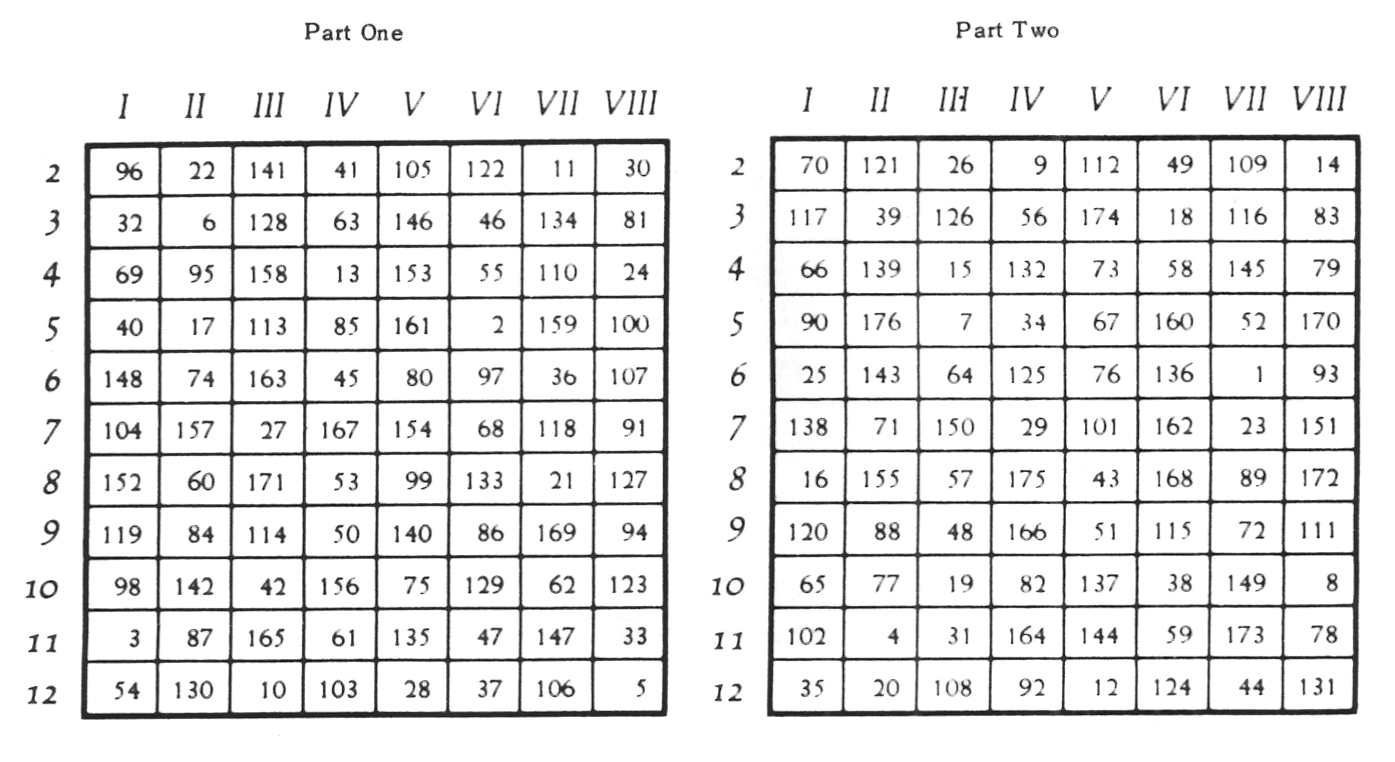
\includegraphics[scale=0.7]{../img/mozart_tables.png}
  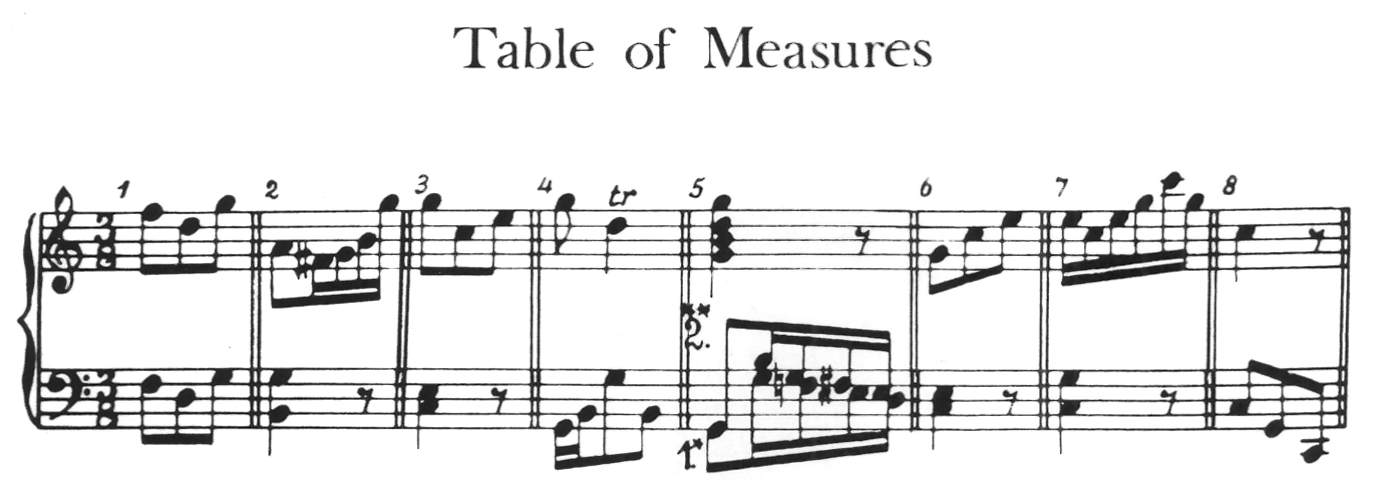
\includegraphics[scale=0.7]{../img/mozart_tables_1.png}
  \end{center}
  
\item music of Changes by J.Cage for piano (1951) in which the formal structure, compositional method and choice of musical materials (pitches, dynamics and tempos) are determined by the roll of the dice of the I-Ching.

  \begin{itemize}
  \tightlist
  \item the collection consists of eight \textit{books} of music.
  \item to compile the score Cage used 8x8 grids (two-dimensional matrices) to facilitate correspondence with the 64 hexagrams of the I Ching.
  \item a first roll of the dice determines which sound event to write among those included in the sound grid, after which the next two rolls are dedicated to durations and dynamics.
  \end{itemize}
  
  \begin{center}
  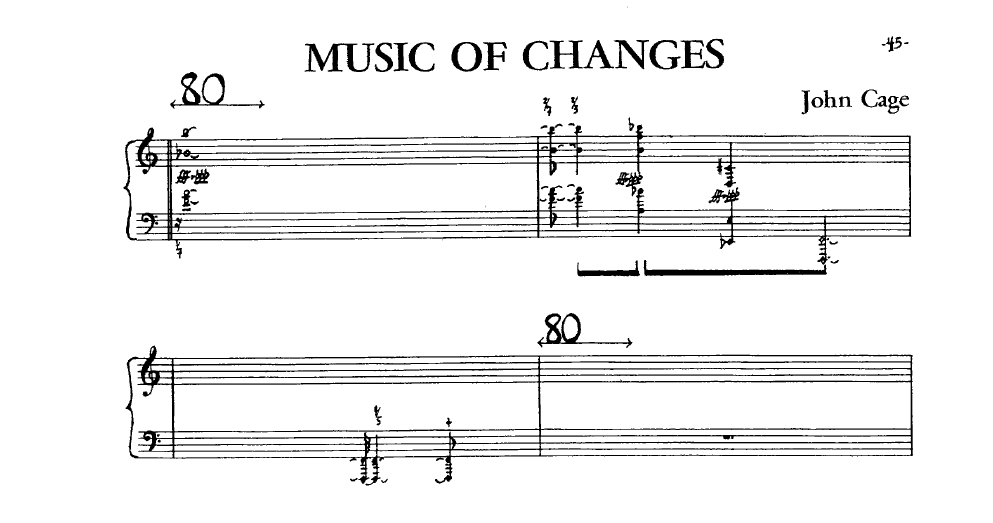
\includegraphics[scale=0.75]{../img/Music_O_C.png}
  \end{center}
\end{itemize}

\subsection{Indeterminacy}\label{indeterminacy}

It seeks the variable multiplicity of possible performances not chance.

Indeterminacy is the opposite of chance which adopts a method.

Chance relies on the logic of the method.

Indeterminacy relies on the performer's sensitivity.

It excludes the precise determination of certain parameters (pitch, duration, intensity, timbre) to give the performer a wide margin of freedom.

When taken to its extreme limits it ideally coincides with the opposite deterministic extreme: total improvisation or \textit{libero arbitrio}.

The concept of indeterminacy in music can be developed in two different ways:

\begin{enumerate}
\def\labelenumi{\arabic{enumi}.}
\tightlist
\item free choice of performance mode or form

  \begin{itemize}
  \tightlist
  \item Missa Cuiusvis Toni (1539) by Johannes Ockeghem.

    \begin{itemize}
    \tightlist
    \item the composer did not specify the clefs at the beginning of the staff.
    \item it can be performed in all four modes (Dorian, Phrygian, Lydian,  Mixolydian).
    \item the choice of which clef to use for reading (and therefore the mode) is left to the performers.
    \end{itemize}
    
    \begin{center}
    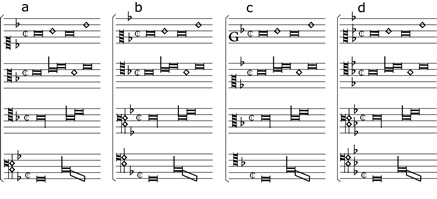
\includegraphics[scale=0.7]{../img/Cuiusvis_toni.png}
    \end{center}
  \item Serenata per un satellite (1969) by B. Maderna

    \begin{itemize}
    \tightlist
    \item It can be played by violin, flute (including piccolo), oboe (including oboe d'amore, even musette), clarinet (transposing the part, of course), marimba, harp, guitar, and mandolin (playing what they can), all together, individually, or in groups, improvising, in short, with the written notes.
    \item the whole piece should last between 4 and 12 minutes.
    \end{itemize}

    \begin{center}
    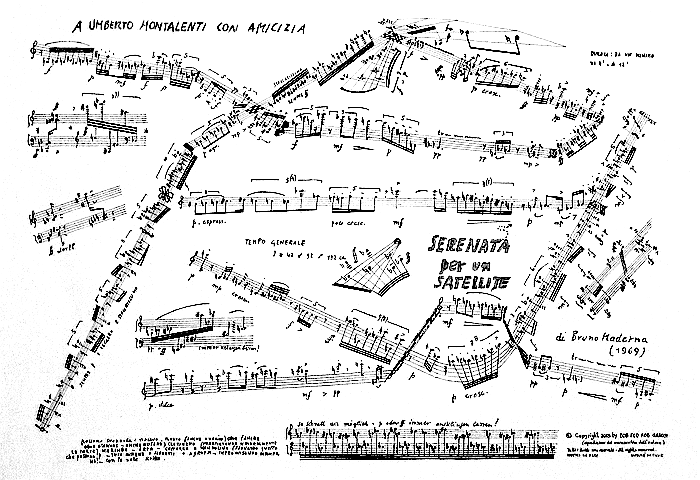
\includegraphics[scale=1]{../img/maderna_1.png}
    \end{center}
  \end{itemize}
\item graphic scores or verbal indications that suggest to the performer how the piece can be performed.

  \begin{itemize}
  \item 4 Systems by Earle Brown.
    \begin{center}
    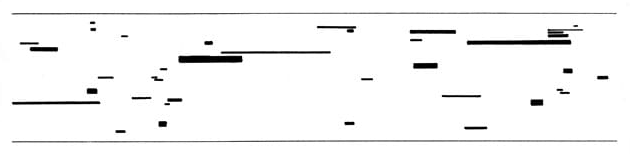
\includegraphics[scale=0.8]{../img/brown1.png}
    \end{center}

  \item Intersection 3 by Morton Feldman (1964).
    \begin{center}
    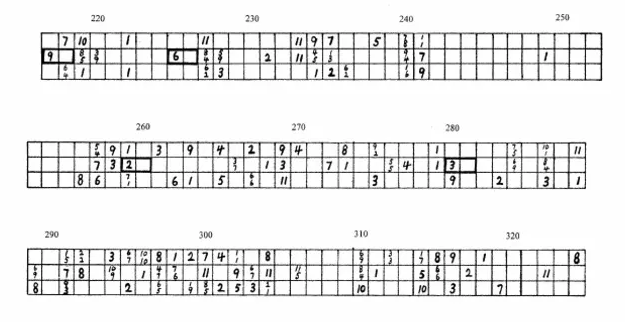
\includegraphics[scale=0.8]{../img/feld.png}
    \end{center}
    
  \item Intuitive Musik (1968) by K.Stockhausen
    \begin{center}
    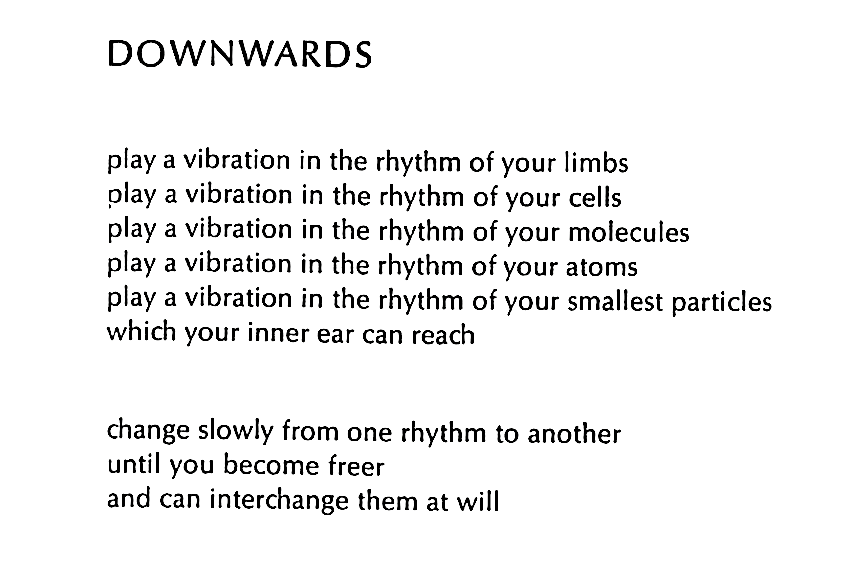
\includegraphics[scale=0.8]{../img/intu.png}
    \end{center}
  \item expressive need - \href{http://www.musicaecodice.it/gitmedia/emc/4_media/maderna1.mp4}{Bruno Maderna} at Venice Biennale
  \end{itemize}
\end{enumerate}

\subsection{Alea}\label{alea}

Aleatoric strategies became common among composers of the European avant-garde.

Acousticist Werner Meyer-Eppler during the Darmstadt summer courses defined it this way:

\textit{A process can be defined as "aleatory" {[}\ldots{]} if its development
is established in general terms but depends on chance in the details}.

Let's explore random procedures in SuperCollider using a SynthDef from previous chapter.

\begin{lstlisting}[frame=single] 
s.boot;
s.meter;
{s.plotTree}.defer(5);
\end{lstlisting}

One Buffer and a SynthDef.

\begin{lstlisting}[frame=single] 
Buffer.freeAll;
b = Buffer.read(s, "/absolute/path/to/file.wav");

SynthDef(\smp, {arg buf=0,pos=0,dur=0.2,amp=0,trsp=0,dir=1,pan=0,
                    t_gate=0,done=2;
                var sig,env;
                    sig = PlayBuf.ar(1, buf,          
                                     BufRateScale.kr(buf) * trsp.midiratio  
                                                          * dir, t_gate,
                                     BufSampleRate.kr(buf)* pos);                  
                    env = Env.linen(0.01,dur-0.02,0.01);                   
                    env = EnvGen.kr(env, t_gate, doneAction:done);
                    sig = Pan2.ar(sig * env * amp, pan);
                Out.ar(0,sig)
        }).add;
\end{lstlisting}

We can obtain random numbers in several ways, here the main objects.

\begin{itemize}
\tightlist
\item boolean \(\rightarrow\) 0.5.coin (0.0 = false, 1.0 = true, 0.x = probability). \\
For example we can use it in a control structure to define the percentage of rests in a sequence.
\pagebreak
\begin{lstlisting}[frame=single, caption=coin(0.5)] 
~rest = 0.8;      // probability of rests in sequence
r = Routine({
            20.do({
                  if(0.8.coin==true) 
                        {Synth(\smp,[\buf,b, \pos,0.23, \amp,1, \dur,0.08,
                                     \pan,0, \t_gate, 1])};
                  0.1.wait;
                  })
                }).reset.play;
\end{lstlisting}

\item within a range (linear distribution) \(\rightarrow\) rrand(min, max). \\
For example we can use it to define random positions in a Buffer.

\begin{lstlisting}[frame=single, caption=rrand(min\,max)] 
~rest = 0.8;        // probability of rests in sequence
~posi = [0.5,3.4];  // start-end position points
r = Routine({
             20.do({
                  if(0.8.coin==true) 
                     {Synth(\smp,[\buf,b, 
                                 \pos, rrand(~posi[0], ~posi[1]), 
                                 \amp, 1, \pan,0, \dur,0.08, \t_gate,1])};
                     0.1.wait})
             }).reset.play;
\end{lstlisting}

\item between 0 and max (linear distribution) \(\rightarrow\) rand(max). \\
For example we can use it to define random amplitude.

\begin{lstlisting}[frame=single, caption=rand(max)] 
~rest = 0.8;       // probability of rests in sequence
~posi = [0.5,3.4]; // start-end position points
r = Routine({
             20.do({
                    if(0.8.coin==true) 
                     {Synth(\smp,[\buf,b, 
                                  \pos, rrand(~posi[0], ~posi[1]),
                                  \amp, rand(1.0),
                                  \pan, 0, \dur,0.08, \t_gate,1])};
                    0.1.wait})
             }).reset.play;
\end{lstlisting}

\item bipolar (linear distribution) \(\rightarrow\) rand2(+/- max)). \\
For example we can use it to define random pan.

\begin{lstlisting}[frame=single, caption=rand2(+/-max)] 
~rest = 0.8;       // probability of rests in sequence
~posi = [0.5,3.4]; // start and end position points
r = Routine({
             20.do({
                    if(0.8.coin==true) 
                     {Synth(\smp,[\buf,b, 
                                  \pos, rrand(~posi[0], ~posi[1]), 
                                  \amp, rand(1.0),
                                  \pan, rand2(1.0),
                                  \dur, 0.08, \t_gate,1])};
                    0.1.wait})
             }).reset.play;
\end{lstlisting}

\item choose in a finite set with a linear distribution \(\rightarrow\)
  {[}3,5,67,89{]}.choose. \\
  For example we can use it to define random choice among a set of durations.

\begin{lstlisting}[frame=single, caption=choose(Array)] 
~rest = 0.8;                 // probability of rests in sequence
~posi = [0.5,3.4];           // start and end position points
~durs = [0.08,0.04,0.2,0.5]; // duration set
r = Routine({
             20.do({
                    if(0.8.coin==true) 
                     {Synth(\smp,[\buf,b, 
                                  \pos, rrand(~posi[0], ~posi[1]),
                                  \amp, rand(1.0),
                                  \dur, ~durs.choose,
                                  \pan, rand2(1.0),
                                  \t_gate, 1]
                    )};
                    0.1.wait;
                    })
             }).reset.play;
\end{lstlisting}
\end{itemize}

There are other objects dedicated to nonlinear distributions but the principles on which they are based are the same as those just illustrated.

\section{Sound synthesis}\label{sound-synthesis}

In this paragraph we will not delve into all the aspects of the individual synthesis techniques.

Only their main sonic and expressive possibilities related to composing music are focused.

Before starting let's define some utility:

\begin{itemize}
\tightlist
\item one SynthDef \(\rightarrow\) set of source signals. 
  \begin{itemize}
  \tightlist
  \item 0 \(\rightarrow\) Live input.
  \item 1 \(\rightarrow\) WhiteNoise.
  \item 2 \(\rightarrow\) Impulse.
  \item 3 \(\rightarrow\) Dust.
  \item 4 \(\rightarrow\) Sawtooth wave.
  \item 5 \(\rightarrow\) Soundfiles player.
  \end{itemize}

  \begin{lstlisting}[frame=single, caption=Source signals model, label=sources] 
SynthDef(\srcs,{arg type=0, freq=400, amp=0, buf=b, busOut=2, gate=0;
                var sig,env;
                    sig =  Select.ar(type,
                                   [SoundIn.ar(0),             // 0
                                    WhiteNoise.ar,             // 1
                                    Impulse.ar(freq),          // 2
                                    Dust.ar(freq),             // 3
                                    Saw.ar(freq),              // 4
                                    PlayBuf.ar(1, buf, loop:1) // 5
                                    ]);
	                env = Linen.kr(gate,doneAction:2);
	                sig = sig * env * amp;
	            Out.ar(busOut, sig)
        }).add;
  \end{lstlisting}

\item one SynthDef \(\rightarrow\) set of control signals (mouse, continuos). 
  \begin{lstlisting}[frame=single] 
SynthDef(\ksig,{arg type=0, range=#[0,1], freq=1, busOut=0;
	            var sig;
	                sig = Select.kr(type,
                                [MouseX.kr(range[0], range[1]),
                                 MouseY.kr(range[0], range[1]),
                                 LFNoise1.kr(freq).range(range[0], range[1])
                                ]);
	            Out.kr(busOut,sig)
        }).add;
  \end{lstlisting}
\item two audio bus to connect the source Synths with filters and FFT Synth. 
\item two control buses to control dynamically parameters (x, y and random signal values). 
\item one spectroscope.

\begin{lstlisting}[frame=single] 
x     = Bus.control(s, 1);   
y     = Bus.control(s, 1);  

s.freqscope;       // a spectroscope
\end{lstlisting}
\end{itemize}

\subsection{Additive}\label{additive}

With additive synthesis techniques we can realize: 

\begin{itemize}
\tightlist
\item harmonic spectra (pitched sounds). 
\item inharmonic spectra (non-pitched sounds).
\end{itemize}

Both categories can have:

\begin{itemize}
\tightlist
\item fixed spectrum.
\item variable spectrum.
\item spectral envelope.
\end{itemize}

There are different ways to do that.

\subsubsection{Wavetables}\label{wavetables}

Harmonic spectra. 

Periodic noises.

Fixed spectrum.

Procedure:
\begin{enumerate}
\tightlist
\def\labelenumi{\arabic{enumi}.}
\item draw a single waveform period.
\item store it in a Buffer.
\item play it back at a defined frequency by an oscillator.
\end{enumerate}

\begin{lstlisting}[frame=single, caption=Wawtable lookup synthesis model] 
SynthDef(\wts, {arg buf=b, freq=500, amp=0, dur=1, t_gate=0, pan=0, done=2;
                var sig,bpf,env;
                    sig = Osc.ar(buf,freq);
                    env = Env.triangle(dur); // change envelope and list
                    env = EnvGen.ar(env,t_gate,doneAction:done);
                    sig = Pan2.ar(sig*amp*env,pan);
	            Out.ar(0,sig)
         }).add;
\end{lstlisting}

We can play it as in previous exemples.

\begin{itemize}
\tightlist
\item deterministic.
\begin{lstlisting}[frame=single] 
Buffer.freeAll;
b = Buffer.alloc(s, 2048);
// Draw Partial_number, magnitudes
b.sine2([1,3,4,6,8,9],[20,30,10,6,7,3].normalizeSum);  
b.plot; 
~pitch = [60,64,65,68,72,73,68,67,60].midicps;
~amps  = [0.3,0.5,0.7,0.3,0.9,0.1]*0.2;
~pans  = [-1,0,1];
~durs  = [0.1,0.5,0.2,0.8,0.4];
~delta = [0.1,0.3,0.1,0.2];

r = Routine({
             20.do({arg i;
                    Synth(\wts,[\buf,b,
			                    \freq, ~pitch.wrapAt(i),
			                    \amp,  ~amps.foldAt(i),
			                    \dur,  ~durs.wrapAt(i),
			                    \pan, ~pans.foldAt(i),
			                    \done,2,
			                    \t_gate,1]); 
                    ~delta.foldAt(i).wait;        
                    })
             }).reset.play;
\end{lstlisting}

\item random.
\begin{lstlisting}[frame=single] 
v = Routine({
	         inf.do({
                     Synth(\wts,[\buf,b,
			                 //  \freq,rrand(50,100).midicps,         // Atonal
			                     \freq, [68,72,75,80].midicps.choose, // Triade
			                     \amp,rand(0.2), 
			                     \dur,rrand(4,8),
			                     \fade,rrand(0.2,8),
			                     \pan, rand2(1.0),
			                     \done,2,
			                     \t_gate,1]);
			         rrand(0.1,2).wait;
			         })
            }).reset.play
\end{lstlisting}
\end{itemize}

\subsubsection{Vectorial}\label{vectorial}

This technique is a variant of wavetable lookup synthesis.

Harmonic spectra.  

Periodic noises.

Variable spectrum.

\begin{enumerate}
\def\labelenumi{\arabic{enumi}.}
\tightlist
\item define an array of different waveforms.
\begin{lstlisting}[frame=single] 
Buffer.freeAll;
b = Buffer.allocConsecutive(4,           // Number of Buffer
                            s, 1024);  
b[0].sine2([1,3,5,7], [1,0.3,0.5,0.7]); // Fill the buffers
b[1].sine2([2,4,6,8], [0.2,0.4,1.3,0.6]);
b[2].sine2([2,3,10,12,13,14], [1,0.2,0.5,0.6,1.3,0.5]);
b[3].sine2([1,3,4,7,8,9,13,18], [1.3,0.3,0.5,0.7,0.8,0.9,0.2,0.3]);
\end{lstlisting}
\item during playback interpolate the reading dynamically with a control parameter.

\begin{lstlisting}[frame=single, caption=Vetorial synthesis model] 
SynthDef(\vec, {arg bufn=4,freq=400,amp=0,pos=0,pan=0,gate=0,done=2;
                var sig,env;
                    sig  = VOsc.ar(pos.linlin(-1,1,0,bufn), freq);
                    env  = Linen.kr(gate,doneAction:done);
                    sig  = Pan2.ar(sig*amp*env,pan);
                Out.ar(0, sig)
                }).add;
\end{lstlisting}
\end{enumerate}

As usual we can change timbre parameter in four different ways.

\begin{enumerate}
\def\labelenumi{\arabic{enumi}.}
\tightlist
\item by sending single values (o to number of buses - 1).
\begin{lstlisting}[frame=single] 
a = Synth(\vec, [\bufn,b.size-1, \freq,400, \amp,0.5, \pan,0, \gate,1]);            
r = Routine({
             5.do({
                   rrand(2,20).do({
                                   a.set(\pos,rand2(1.0));
                                   0.1.wait});
                   rrand(0.2,1).wait});
                   a.free;
             }).reset.play;
\end{lstlisting}

\item by mapping a control signal on a control bus as argument.
\begin{lstlisting}[frame=single] 
k = Synth(\ksig, [\type,0, \range,[-1, 1], \busOut, x]); // Mouse x  
a = Synth(\vec,  [\bufn,b.size-1, \freq,400, \pos, x.asMap, 
                  \amp,0.5, \pan,0, \gate,1]);
\end{lstlisting}

Change the control signal type and sub-audio frequency.

\begin{lstlisting}[frame=single] 
k.set(\type,2, \freq,1);
\end{lstlisting}
\end{enumerate}

Another classic technique in digital synth design is to map the amplitude envelope with spectral modification.

A simulation of acoustic natural sounds.

\begin{lstlisting}[frame=single,caption=Envelope mapping parameter] 
SynthDef(\vmap, {arg buf=0,bufn=4,freq=400,dur=1,amp=0,pan=0,t_gate=0,done=2;
                 var sig,bpf,env;
                     bpf   = Env.sine(dur);
                     env   = EnvGen.ar(bpf,t_gate,doneAction:done);
                     sig   = VOsc.ar(env.linlin(0,1,buf,bufn-1), freq);
                     sig   = Pan2.ar(sig*amp*env,pan);
                 Out.ar(0, sig)
         }).add;
\end{lstlisting}

Play it.

\begin{lstlisting}[frame=single] 
r = Routine({
             10.do({
                    Synth(\vmap, [\buf,b, \bufn,3,
                                  \freq,rrand(40, 76).midicps,
                                  \dur,rrand(4,12),
                                  \amp,rand(1.0),
                                  \pan,rand2(1.0),
                                  \t_gate,1]);
                    rrand(3,5).wait;
                    })
             }).reset.play;
\end{lstlisting}

\subsubsection{PWM}\label{pwm}

Pulse Width Modulation.

This technique is a variant of wavetable lookup synthesis and allows the generation of variable spectra.

Harmonic spectra.

Variable spectrum.

It is based on the concept of duty cycle.

\begin{center}
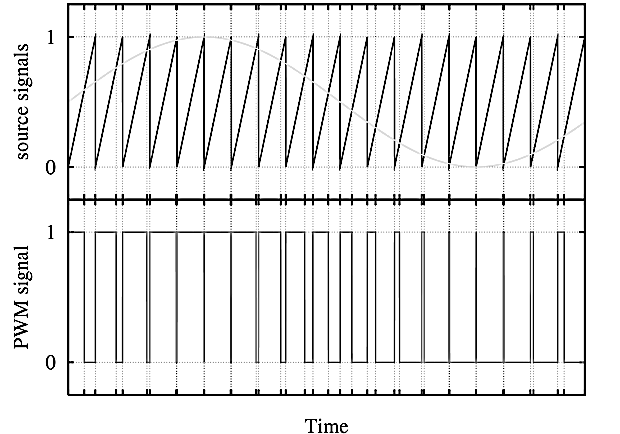
\includegraphics[scale=0.7]{../img/pwm.png}
\end{center}

By changing this parameter we modify the timbre.

\begin{lstlisting}[frame=single, caption=Pulse Width Modulation model] 
SynthDef(\pwm, {arg freq=300,duty=0.5,amp=0,gate=0,pan=0,done=2;
                var sig, env;
                    sig  = Pulse.ar(freq, duty);
                    env  = Linen.kr(gate,doneAction:done);	               
                    sig  = Pan2.ar(sig * amp * env,pan);
                Out.ar(0,sig)
         }).add;
\end{lstlisting}

The Synth.

\begin{lstlisting}[frame=single] 
a = Synth(\pwm, [\amp,0.5,\duty,1/2,\gate,1]);
\end{lstlisting}

We can change the duty cycle from 0.0 to 0.5.

Let's observe how the spectrum changes by set 1/3, 1/4, 1/5 etc.

\begin{lstlisting}[frame=single] 
a.set(\duty, 1/4);
\end{lstlisting}

Duty cycle and other parameter control methods are the same as those illustrated previously.

Some variations of this technique.

Blip \(\rightarrow\) classic pulse train derived from MusicN languages
(buzz) implemented in commercial synthesizers of the 90s.

We can define the number of harmonics as an argument.

\begin{lstlisting}[frame=single, caption=Blip model] 
SynthDef(\blip,{arg freq=300,nharm=20,amp=0,gate=0,pan=0,done=2;
                var sig,env;
                    sig   = Blip.ar(freq, nharm); 
                    env   = Linen.kr(gate,doneAction:done);
                    sig   = Pan2.ar(sig*amp*env,pan);
                Out.ar(0,sig)
         }).add;
\end{lstlisting}

The sequence.

\begin{lstlisting}[frame=single] 
a = Synth(\blip, [\amp,0.5,\gate,1]);                   
r = Routine({
             10.do({
                    rrand(2,10).do({
                                    a.set(\freq, [50,57,62].midicps
                                                           .choose
                                          \nharm,rrand(1,30));
                                    0.1.wait;
                                    });
                    0.2.wait;
                    });
             a.set(\gate,0);
             }).reset.play;
\end{lstlisting}

Control signal.

\begin{lstlisting}[frame=single] 
k = Synth(\ksig, [\type,2, \range, [1, 20], \freq,1, \busOut, x]);
a = Synth(\blip, [\amp,0.5, \nharm, x.asMap, \gate,1])
\end{lstlisting}

We can also realize PWM with different waveforms stored in a Buffer (timbre stretching).

\begin{lstlisting}[frame=single, caption=Timbre stretching model] 
SynthDef(\wsth,{arg buf=b, freq=500, sfact=1, amp=0,gate=0,pan=0,done=0;
                var p,f,c,sig,env;
                    p   = BufFrames.kr(buf);  
                    f   = sfact;
                    c   = LFSaw.ar(freq) *  0.5 * p * f + (p * 0.5);	               
                    sig = BufRd.ar(1,buf,c,1,4);
                    env = Linen.kr(gate,doneAction:done);
                    sig = Pan2.ar(sig*amp*env,pan);
                Out.ar(0,sig)
         }).add;
\end{lstlisting}

The Synths.

\begin{lstlisting}[frame=single] 
Buffer.freeAll;
b = Buffer.alloc(s, 2048);
b.sine2([1,3,4,6,8,9],                 // Draw Partial_number
        [20,30,10,6,7,3].normalizeSum, // magnitudes
        asWavetable: false); 
        
k = Synth(\ksig, [\type,0, \range, [1,10], \freq,1, \busOut, x]);
a = Synth(\wsth, [\buf,b,\freq,100,\amp,0.12,\sfact,x.asMap,\done,2,\gate,1]);
\end{lstlisting}

\subsubsection{Classic}\label{classic}

Harmonic spectra.

Inharmonic spectra.

Spectral envelope.

The techniques just described belong to the world of digital audio.

In the early electroacoustic music studios (Cologne and Milan), additive synthesis was achieved by recording each individual partial and then mixing it with the others.

Let's simulate this process defining a SynthDef that play only a single partial.

\begin{lstlisting}[frame=single, caption=Partial model] 
SynthDef(\par, {arg freq=500,amp=0,pha=0,dur=1,pan=0,t_gate=0;
                var sig, env;
                    sig = SinOsc.ar(freq, pha, amp);      
                    env = Env.perc(0.1*dur,0.9*dur);
                    env = EnvGen.ar(env, t_gate, doneAction:2);
                    sig = sig * env;
                    sig = Pan2.ar(sig, pan);
         Out.ar(0, sig)
         }).add;
\end{lstlisting}

Then we can define spectra as Arrays and play it through a loop structure.

\begin{lstlisting}[frame=single] 
//~freqs = [1,   3,   4,   5,    8]* 52.midicps;   // Harmonic
~freqs = [1169,1733,854, 1596, 1480];              // Inharmonic
~amps  = [10,  100,  80,   30,  171].normalizeSum; // Amplitudes (sum=1)
~dur   = 3;                                        // Overall duration
~durs  = [0.1, 0.8,  0.5, 0.3,  1.0] * ~dur;       // Partials durations              

~freqs.size.do({arg i;      // loop without .wait
                Synth(\par, [\freq, ~freqs[i],
                      \amp,  ~amps.at(i),
                      \dur,  ~durs[i],
                      \t_gate,1])
                })
\end{lstlisting}

Deterministic sequence.

\begin{lstlisting}[frame=single] 
~seq = [60,  64, 67, 68, 71, 72].scramble.midicps;
~amp = [0.9,0.7,0.5,0.3,0.2,0.1].scramble;
~dur = [0.1,0.4,0.2,0.8,0.5,  1].scramble;
g    = ~seq.size;

u = Routine({var parz, pamp, pdur;
                 parz = [ 1,   3,  4,  5,  8];  // Spectrum
                 pamp = [10, 100, 80, 30,171].normalizeSum;
                 pdur = [0.1,0.8,0.5,0.3,1.0]; 
                 h    = parz.size;
             g.do({arg i;
                   var freq, amps, durs;
                       freq = parz * ~seq[i];   
                       amps = pamp * ~amp[i];
                       durs = pdur * ~dur[i];
                       h.do({arg i;
                             Synth(\par,[\freq, freq[i],
                                         \amp,  amps[i],
                                         \dur,  durs[i],
                                         \t_gate, 1])
                             });
                       0.1.wait;              
                   })
             }).reset.play;
\end{lstlisting}

Random sequence - difference between chords and spectra.

\begin{lstlisting}[frame=single] 
~bpm = 72;
t = TempoClock.new(~bpm/60); 
r = Routine({
             inf.do({var nharm;
                     if(0.2.coin==false) // Random rest percentage
                     {nharm = rrand(2,9);
                      nharm.do({arg i;
                                Synth(\par,[\freq, [70,74,75,78,82,86,90].midicps.choose, 
                                      \amp,  rand(1/nharm),
                                      \dur,  [0.05,0.2,0.4].choose,
                                      \pan, [-1,1].choose,
                                      \t_gate,1])
                                });
                      };
                      [0.125,0.25].choose.wait;              
                     })
             }).reset.play(t);
\end{lstlisting}

\subsection{Subtractive}\label{subtractive}

Sound source ranging from white noise to rich spectra filtered by one or more filter(s).

Main types:

\begin{enumerate}
\tightlist
\item Low Pass Filter (LPF) 
\item High Pass Filter (HPF) 
\item Band Pass Filter (BPF) 
\item Band Reject Filter (BRF) 
\item Resonant Filter (Resonz)
\end{enumerate}

In SuperCollider are all 2nd order \href{http://www.musicaecodice.it/gitmedia/emc/4_media/Butterworth_filters.pdf}{Butterworth filters} (-12 dB/oct).

We can control cut/central frequency (Hz).

In BPF, BRF and Resonz we can also control the bandwidth (reciprocal of Q).

\begin{itemize}
\tightlist 
\item low values \(\rightarrow\) narrow band. 
\item high values \(\rightarrow\) wide band.
\end{itemize}


Sources can be chosen with \textit{Source signals model} (\ref{sources}) already defined previously.

Filters can be defined with dedicated SynthDefs (one for each filter type).

\begin{itemize}
\tightlist 
\item the first we can set audio Bus out.
\item the second audio Bus in.
\end{itemize}

In SuperCollider there are many audio buses.

In a stereo system: 

\begin{itemize}
\tightlist 
\item public buses \(\rightarrow\) 0 and 1 (L and R) 
\item private buses \(\rightarrow\) 2 and up.
\end{itemize}

A simple signal flow.

\begin{center}
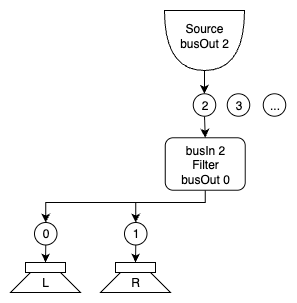
\includegraphics[scale=0.75]{../img/filt_1.png}
\end{center}

\begin{lstlisting}[frame=single, caption=Filters models] 
SynthDef(\lpf, {arg freq=500, amp=0, busIn=2, busOut=0, pan= -1;
                var sig;
                    sig = In.ar(busIn);
                    sig = LPF.ar(sig, freq) * amp;
                    sig = Pan2.ar(sig, pan);
                Out.ar(busOut, sig)
         }).add;
SynthDef(\hpf, {arg freq=500, amp=0, busIn=2, busOut=0, pan= -1;
                var sig;
                    sig = In.ar(busIn);
                    sig = HPF.ar(sig, freq) * amp;
                    sig = Pan2.ar(sig, pan);
                Out.ar(busOut, sig)
         }).add;
SynthDef(\bpf, {arg freq=500, amp=0, bw=1, busIn=2, busOut=0, pan= -1;
                var sig;
                    sig = In.ar(busIn);
                    sig = BPF.ar(sig, freq) * amp;
                    sig = Pan2.ar(sig, pan);
                Out.ar(busOut, sig)
         }).add;
SynthDef(\brf, {arg freq=500, amp=0,  bw=1, busIn=2, busOut=0, pan= -1;
                var sig;
                    sig = In.ar(busIn);
                    sig = BRF.ar(sig, freq) * amp;
                    sig = Pan2.ar(sig, pan);
                Out.ar(busOut, sig)
         }).add;
SynthDef(\res, {arg freq=500, amp=0,  bw=1, busIn=2, busOut=0, pan= -1;
                var sig;
                    sig = In.ar(busIn);
                    sig = Resonz.ar(sig, freq) * amp;
                    sig = Pan2.ar(sig, pan);
                Out.ar(busOut, sig)
         }).add;
\end{lstlisting}

The Synths (in right order).

\begin{enumerate}
\tightlist 
\item signal.
\item filter.
\end{enumerate}

Here we set creation order with \textit{addToTail} command.

\begin{lstlisting}[frame=single] 
Buffer.freeAll;
b = Buffer.read(s, "/absolute/path/to/file.wav"); // for source Synth

a = Synth(\srcs, [\type,1, \buf,b, \amp,1, \busOut,12, \gate,1]);
f = Synth(\lpf,  [\freq,1000, \amp,1, \busIn,12, \busOut,0, \pan, -1], 
          s, \addToTail);
\end{lstlisting}

Change the filter cutting frequency parameter in the usual ways.

\begin{lstlisting}[frame=single] 
f.set(\freq, rrand(200,2000).postln);
\end{lstlisting}

We can sculpt the spectrum using filter banks in two combinations:

\begin{enumerate}
\def\labelenumi{\arabic{enumi}.}
\tightlist
\item series \(\rightarrow\) output of one filter is the input of the next until the public output.
\begin{lstlisting}[frame=single] 
a = Synth(\srcs, [\type,5,\buf,b,\amp,1,\busOut,12,\gate,1]);
b = Synth(\lpf, [\freq,100,\amp,0.6,\busIn,12,\busOut,13,\pan,-1],
          s,\addToTail);
c = Synth(\brf, [\freq,800,\bw,2,\amp,0.6,\busIn,13,\busOut,14,\pan,-1],
          s,\addToTail);
d = Synth(\brf, [\freq,800,\bw,1,\amp,2.5,\busIn,14,\busOut,0,\pan,0],
          s,\addToTail);
                    
r = Routine({
            inf.do({
                    b.set(\freq, rrand(8000,12000)); 
                    c.set(\freq, rrand(200,1000));
                    d.set(\freq, rrand(800,3000));
                    0.25.wait;
                    })
            }).reset.play
\end{lstlisting}

\item parallel \(\rightarrow\) output of source is the input of all filters, ouputs of filters mix together.
\begin{lstlisting}[frame=single] 
~bw     = 0.1;    // Try to change
~amp    = 1;
~source = 5;
~rib    = 0.1;

a = Synth(\srcs, [\type,~source,\buf,b,\amp,1,\busOut,12,\gate, 1]);
b = Synth(\bpf, [\freq,100,\bw,~bw,\amp,~amp,\busIn,12,\busOut,0,\pan,-1],
          s,\addToTail);
c = Synth(\bpf, [\freq,800,\bw,~bw,\amp,~amp,\busIn,12,\busOut,0,\pan,-1],
          s,\addToTail);
d = Synth(\bpf, [\freq,800,\bw,~bw,\amp,~amp,\busIn,12,\busOut,0,\pan,0],
          s,\addToTail);
                    
r = Routine({
            inf.do({
                    b.set(\freq, rrand(100,700)); 
                    c.set(\freq, rrand(1700,2100));
                    d.set(\freq, rrand(3000,3100));
                    ~rib.wait;
                    })
            }).reset.play
\end{lstlisting}

\end{enumerate}

In SuperCollider there are also pre builded filterbanks which can be used to simulate an object's resonant modes.

We can set for each resonance:
\begin{itemize}
\tightlist
\item frequencies.
\item amplitudes.
\item duration.
\end{itemize}

\begin{lstlisting}[frame=single, caption=Resonators model] 
SynthDef(\reson, {arg freqs=#[800, 1071, 1153, 1723],
                      amps=#[0.1,0.1,0.1,0.1],
                      ringtimes=#[1, 1, 1, 1],
                      busIn=2,
                      busOut=0,
                      pan=0;
                  var in, sig;
                      in  = In.ar(busIn);
                      sig = DynKlank.ar(`[freqs, amps, ringtimes ], in);
                      sig = Pan2.ar(sig, pan); 
                  Out.ar(busOut, sig);
         }).add;
\end{lstlisting}

The Synths.

\begin{lstlisting}[frame=single] 
e = Synth(\srcs,  [\type, 2,\freq,3,\amp,0.5,\busOut,12,\gate,1]);
a = Synth(\reson, [\busIn,12, \busOut,0,\pan,0], s, \addToTail);
\end{lstlisting}

Change resonator parameter.

\begin{lstlisting}[frame=single] 
a.setn(\freqs, Array.rand(4, 500, 9000));
a.setn(\amps, Array.rand(4, 0.1, 1));
a.setn(\ringtimes, Array.rand(4, 0.2, 2.4) );
\end{lstlisting}

Change source. 

\begin{enumerate}
\def\labelenumi{\arabic{enumi}.}
\tightlist
\item \(\rightarrow\) White Noise. 
\item \(\rightarrow\) Impulse
\item \(\rightarrow\) Dust.
\end{enumerate}

\begin{lstlisting}[frame=single] 
e.set(\type,3,\amp,0.1);
\end{lstlisting}

Be careful with amplitude.

\subsection{FM}\label{fm}

In additive synthesis and in some cases in subtractive synthesis the signals are added together to obtain complex spectra.

The computational cost is high since for each partial or filter we have to generate a UGen.

Through the different basic modulation techniques (RM, AM, FM and PM) we can obtain equally rich spectra with only two signals: 

\begin{itemize}
\tightlist 
\item carrier. 
\item modular.
\end{itemize}

In this paragraph we explore characteristics of frequency modulation in its most basic form.

We use a rescaled sinusoidal control signal (modular) to vary the frequency of a sinusoid (carrier).

Three parameters:

\begin{itemize}
\tightlist 
\item  carrier frequency. 
\item modular frequency.
\item deviation from carrier frequency (ampitude of modular signal).
\end{itemize}

If the frequency of modular signal is sub audio and deviation is under \textasciitilde5 Hz \(\rightarrow\) \textit{vibrato effect}.

\begin{lstlisting}[frame=single, caption=Basic FM model] 
SynthDef(\fm_bas, {arg carf=440;
                   var modf, dev, mod, car;
                       modf = MouseX.kr(1,500);
                       dev  = MouseY.kr(1,500);
                       mod = carf + (SinOsc.ar(modf) * dev);
                       car = SinOsc.ar(mod);
                   Out.ar(0,car*0.3)
                 }).add;
\end{lstlisting}

The Synth.

\begin{lstlisting}[frame=single] 
a = Synth(\fm_bas);
\end{lstlisting}

We can already recognize the characteristic sound of this technique.

In classic FM algorithm we can control:

\begin{itemize}
\tightlist 
\item carrier frequency.
\item modulation index \(\rightarrow\) quantity of modulation. 
\item harmonicity index \(\rightarrow\) quality of modulation.
\end{itemize}

We can realize a lot of different sounds changing only these two parameters.

\begin{lstlisting}[frame=single, caption=Classic FM model] 
SynthDef(\fm, {arg freq=440, amp=0, hid=0, mid=0, smth=0.001, pan=0, gate=0;
               var fmod, mod, por, env, sig;
                   fmod = freq * hid.round(smth);
                   mod  = freq + (SinOsc.ar(fmod) * fmod * mid);
                   por  = SinOsc.ar(mod);
                   env  = Linen.kr(gate, doneAction:2);
                   sig  = por * amp * env;
                   sig  = Pan2.ar(sig, pan);
               Out.ar(0, sig)
         }).add;
\end{lstlisting}

Let's explore it with mouse position using the SynthDef already defined (\ref{control}).

\begin{lstlisting}[frame=single] 
k = Synth(\ksig, [\type,0, \range, [0, 15], \busOut, x]); // Harmonicity index
j = Synth(\ksig, [\type,1, \range, [0, 25], \busOut, y]); // Modulation index
a = Synth(\fm,   [\freq,200, \amp,0.4, \hid,x.asMap, \mid,y.asMap, \gate,1]);
\end{lstlisting}

I suggest exploring the sonic potential of this technique empirically through mouse controls.

\begin{enumerate}
\tightlist 
\item move the mouse. X and y positions can be dynamically reported in the Post window with \textit{.poll} method invoked on MouseX.kr and MouseY.kr UGens in \textit{ksig} SynthDef.

\item hear an intresting sound and write the values.

\item recall them in a deterministic way eventually interpolating them with other sounds through envelopes or other kind of controls.
\end{enumerate}

In this way we can realize different musical objects fixing deterministic values with an empirical interactive strategy.

An exemple. 

Let's define a SynthDef for envelope contol.

\begin{lstlisting}[frame=single, caption=Envelope control model] 
SynthDef(\env, {arg levels=#[0,1,0.5,0.7,0], times=#[1,1,1,1], dur=1, 
                    busOut=0, t_gate=0;
                var env;
                    env = Env.new(levels,times.normalizeSum * dur);
                    env = EnvGen.kr(env, t_gate);
                Out.kr(busOut,env)
         }).add;
\end{lstlisting}

The Synths.

\begin{lstlisting}[frame=single] 
h = Synth(\env,[\levels, [3.5,3.4,3.6,3.7,3.35],  // Harmonicity index
                \times,  [3,4,2,5],
                \dur, 40,
                \busOut, x]); // write on control bus
i = Synth(\env,[\levels, [0,1,0.5,1.2,0.7],       // Modulation index
                \times,   [1,4,9,5],
                \dur, 42,
                \busOut, y]); // write on control bus

a = Synth(\fm, [\freq,100, \amp,0.4, \hid,x.asMap, \mid,y.asMap]);
                
r = Routine.new({
                 a.set(\gate,1);
                 h.set(\t_gate,1); 
                 i.set(\t_gate,1);
                 50.wait; 
                 a.release(8);h.free;i.free;k.free;j.free;
                 }).reset.play
\end{lstlisting}

\subsection{FFT}\label{fft}

Some classical techniques related to the analysis and resynthesis via the Fast Fourier Transform.

We analyze a signal by transforming it from time to frequency domain obtaining values of:

\begin{itemize}
\tightlist 
\item magnitude.
\item phase.
\end{itemize}

of a set of equidistant frequencies (bins) within the spectrum (as teeth of a comb).

We can manipulate these values in various ways and then bring them back into the time domain.

Two main procedures:

\begin{itemize}
\tightlist 
\item analyze, process, and resynthesize a single signal. 
\item analyze two signals, combine the data in various ways and resynthesize the result.
\end{itemize}

In SuperCollider there ia a set of classes dedicated to Phase Vocoder which is a historical FFT analysis and resynthesis technique.

To use classes in these examples download and install \href{https://supercollider.github.io/sc3-plugins/}{sc3-plugins}.

Be careful because FFT processes are CPU expensive.

In all the exemples we use the previous defined \textit{source signal model} (\ref{sources}) and \textit{control signal model} (\ref{control}) SynthDefs.

\subsubsection{Spectral Delay}\label{spectral-delay}

Change delay time without pitch artefacts.

\begin{lstlisting}[frame=single,caption=Spectral Delay model] 
SynthDef(\sdel,{arg busIn=0,busOut=0,amp=0.5,fadeT=0.5,gate=0,pan=0,
                    maxdel=1,del= 0;
                var in,size,chain,env,sig;
                    in    = In.ar(busIn,1);
                    size  = 2048;
                    chain = FFT(LocalBuf(size), in); // analysis
                    chain = chain.pvcollect(size, {arg mag,fasi,bin;  
   [mag + DelayN.kr(mag, maxdel, del.linlin(0,1,0,maxdel)), // process 
    fasi] },0,256,-1);
                    env = Linen.kr(gate,fadeT,1,fadeT,doneAction:2);
                    sig = IFFT(chain) * env * amp;   // resyntesis
                    sig = Pan2.ar(sig, pan);
                Out.ar(busOut, sig);
         }).add;
\end{lstlisting}

The Synths.

\begin{lstlisting}[frame=single] 
Buffer.freeAll;
b = Buffer.read(s, "/absolute/path/to/file.wav");

k = Synth(\ksig, [\type, 0, \range, [0, 1], \busOut,x]); // Normalized
e = Synth(\srcs, [\type, 5, \amp,1, \buf,b, \busOut,12, \gate,1 ],
          s,\addToTail);
a = Synth(\sdel, [\busIn,12, \amp,1, \maxdel,5, \del,x.asMap, \gate,1],
          s,\addToTail);
\end{lstlisting}

\subsubsection{Brick Wall filter}\label{brickwall-filter}

Only bins above or below a threshold between +/-1 pass.

We can define ideal low and high pass filters.

\begin{lstlisting}[frame=single, caption=Brick Wall spectral filter model] 
SynthDef(\bwall, {arg busIn=0,busOut=0,amp=0.5,fadeT=0.5,gate=0,pan=0,
                      lpf=20000,hpf=20;
                      var in,size,chain,env,sig;
                      in    = In.ar(busIn,1);
                      size  = 2048;
                      chain = FFT(LocalBuf(size), in);
          chain = PV_BrickWall(chain, lpf.linlin(20,20000,-1,0)); // LPF
          chain = PV_BrickWall(chain, hpf.linlin(20,20000,0,1));  // HPF
                      env   = Linen.kr(gate,fadeT,1,fadeT,doneAction:2);
                      sig   = IFFT(chain) * env * amp;
                      sig   = Pan2.ar(sig, pan);
                  Out.ar(busOut, sig);
         }).add;
\end{lstlisting}

The Synths.

\begin{lstlisting}[frame=single] 
e = Synth(\srcs,  [\type, 5,  \amp,1, \buf,b, \busOut,12, \gate,1 ]);
a = Synth(\bwall, [\busIn,12, \amp,1, \lpf,6000, \hpf, 1000, \gate,1],
          s,'addToTail');
\end{lstlisting}

Change filter freqs.

\begin{lstlisting}[frame=single] 
a.set(\lpf, 500, \hpf,200);
\end{lstlisting}

Dynamically (mouse x and y).

\begin{lstlisting}[frame=single] 
k = Synth(\ksig, [\type,0, \range, [500,10000], \busOut,x]);
j = Synth(\ksig, [\type,0, \range, [200, 1000], \busOut,y]);
a.set(\lpf, x.asMap, \hpf, y.asMap);
\end{lstlisting}

\subsubsection{Rect Comb filter}\label{rect-comb-filter}

Make gaps in spectrum.

\begin{itemize}
\tightlist 
\item teeth \(\rightarrow\) number of teeth in the comb. 
\item fase \(\rightarrow\) starting phase of comb pulse. 
\item width \(\rightarrow\) pulse width of the comb.
\end{itemize}

\begin{lstlisting}[frame=single,caption=Rect Comb filter spectral model] 
SynthDef(\rcomb, {arg busIn=0,busOut=0,amp=0.5,fadeT=0.5,gate=0,pan=0,
                      teeth=10,fase=0,width=0.5;
                  var in,size,chain,env,sig;
                      in    = In.ar(busIn,1);
                      size  = 2048;
                      chain = FFT(LocalBuf(size), in);
                      chain = PV_RectComb(chain, teeth, fase, width);
                      env   = Linen.kr(gate,fadeT,1,fadeT,doneAction:2);
                      sig   = IFFT(chain) * env * amp;
                      sig   = Pan2.ar(sig, pan);
                  Out.ar(busOut, sig);
         }).add;
\end{lstlisting}

The Synths.

\begin{lstlisting}[frame=single] 
e = Synth(\srcs,  [\type, 5, \amp,1, \buf,b, \busOut,12, \gate,1 ]);
a = Synth(\rcomb, [\busIn,12, \amp,1, \gate,1],s,'addToTail');
\end{lstlisting}

Change phases.

\begin{lstlisting}[frame=single] 
a.set(\fase,rand(1.0).postln);
\end{lstlisting}

Change width and teeth dynamically.

\begin{lstlisting}[frame=single] 
k = Synth(\ksig, [\type,0, \range, [0.01, 0.5], \busOut,x]);
j = Synth(\ksig, [\type,0, \range, [1, 30], \busOut,y]);
a.set(\width, x.asMap, \teeth, y.asMap);
\end{lstlisting}

\subsubsection{Mag Smear}\label{mag-smear}

Average magnitudes across bins, we can set the number of bins to average on each side of bin.

\begin{lstlisting}[frame=single,caption=Mag Smear spectral model] 
SynthDef(\smear, {arg busIn=0,busOut=0,amp=0.5,fadeT=0.5,gate=0,pan=0,
                      bins=1;
                  var in,size,chain,env,sig;
                      in    = In.ar(busIn,1);
                      size  = 2048;
                      chain = FFT(LocalBuf(size), in);
                      chain = PV_MagSmear(chain, bins);
                      env   = Linen.kr(gate,fadeT,1,fadeT,doneAction:2);
                      sig   = IFFT(chain) * env * amp;
                      sig   = Pan2.ar(sig, pan);
                  Out.ar(busOut, sig);
         }).add;
\end{lstlisting}

The Synths.

\begin{lstlisting}[frame=single] 
k = Synth(\ksig,  [\type,0, \range, [0, 10], \busOut,x]);
e = Synth(\srcs,  [\type, 5, \amp,1, \buf,b, \busOut,12, \gate,1 ]);
a = Synth(\smear, [\busIn,12, \amp,1, \bins, x.asMap, \gate,1],s,'addToTail');
\end{lstlisting}

\subsubsection{Freeze}\label{freeze}

Freeze magnitudes when freeze argument \textgreater{} 0.

\begin{lstlisting}[frame=single,caption=Freeze spectral model] 
SynthDef(\frz, {arg busIn=0,busOut=0,amp=0.5,fadeT=0.5,gate=0,pan=0,
                    frz=0;
                var in,size,chain,env,sig;
                    in    = In.ar(busIn,1);
                    size  = 2048;
                    chain = FFT(LocalBuf(size), in);
                    chain = PV_MagFreeze(chain, frz);
                    env   = Linen.kr(gate,fadeT,1,fadeT,doneAction:2);
                    sig   = IFFT(chain) * env * amp;
                    sig   = Pan2.ar(sig, pan);
                Out.ar(busOut, sig);
         }).add;
\end{lstlisting}

The Synths and the sequence.

\begin{lstlisting}[frame=single] 
e = Synth(\srcs, [\type, 5, \amp,1, \buf,b, \busOut,12, \gate,1 ]);
a = Synth(\frz,  [\busIn,12, \amp,1, \gate,1],s,'addToTail');
                    
r = Routine({
             10.do({a.set(\frz,0);
                    rrand(0.2,2).wait;
                    a.set(\frz,1);
                    rrand(0.6,2).wait;
                    });
             e.set(\gate,0); a.set(\gate,0);    
             }).reset.play;
\end{lstlisting}

\subsubsection{Cross synthesys.}\label{cross-synthesys.}

There are several cross-synthesis techniques.

In this example the bins of signal A are replaced by those of signal B.

\begin{lstlisting}[frame=single,caption=Morphing spectral model] 
SynthDef(\cross, {arg busIn=#[0,1],busOut=0,amp=0.5,fadeT=0.5,gate=0,pan=0,
                      morph=0;
                  var inA,inB,size,chainA,chainB,chain,env,sig;
                      inA    = In.ar(busIn[0],1);
                      inB    = In.ar(busIn[1],1);
                      size   = 2048;
                      chainA = FFT(LocalBuf(size), inA);
                      chainB = FFT(LocalBuf(size), inB);
                      chain  = PV_Morph(chainA, chainB, morph);
                      env    = Linen.kr(gate,fadeT,1,fadeT,doneAction:2);
                      sig    = IFFT(chain) * env * amp;
                      sig    = Pan2.ar(sig, pan);
                  Out.ar(busOut, sig);
         }).add;
\end{lstlisting}

The Synths (two different sources).

\begin{lstlisting}[frame=single] 
k = Synth(\ksig,  [\type,0, \range, [0, 1.0],    \busOut,x]);
e = Synth(\srcs,  [\type, 5, \amp,1, \buf,b,     \busOut,12, \gate,1 ]);
g = Synth(\srcs,  [\type, 2, \amp,0.8, \freq, 8, \busOut,13, \gate,1 ]);
a = Synth(\cross, [\busIn,[12, 13], \amp,1, \morph, x.asMap, \gate,1],
          s,'addToTail');
\end{lstlisting}

\section{Algorithmic structures}\label{algorithmic-structures}

In this chapter we expanded our sonic vocabulary.

We can now design formal structures by adopting the same strategies illustrated in the previous chapter or through non-deterministic algorithms.

Let's give an example of this second case.

Suppose we want to create a piece with dreamlike feeling based on three musical objects:

\begin{enumerate}
\def\labelenumi{\arabic{enumi}.}
\tightlist
\item continuos changing crystal sounds (filter bank). 
\item short sequences of percussive brilliant sounds (vector synth). 
\item a strange piano (FFT filter).
\end{enumerate}

For each we define one SynthDef, a function and a score sequence.

\begin{enumerate}
\def\labelenumi{\arabic{enumi}.}
\tightlist
\item continuos changing crystal sounds.

\begin{lstlisting}[frame=single] 
SynthDef(\res, {arg freqs=#[800, 1071, 1153, 1723],
                    amps=#[0.1,0.1,0.1,0.1],
                    ringtimes=#[1, 1, 1, 1],
                    busOut=0, gate=0;
                var sig, amp, env, pan;
                    sig = WhiteNoise.ar;  
                    amp = LFNoise1.kr(0.2).range(0,0.07); 
                    sig = sig * amp;      
                    sig = DynKlank.ar(`[freqs, amps, ringtimes ], sig);
                    env = Linen.kr(gate, 3, doneAction:2);
                    pan = LFNoise1.kr(0.3);          
                    sig = Pan2.ar(sig * amp * env, pan); 
                Out.ar(busOut, sig);
}).add;
// Define the musical object
a = {Routine({var fqs, aps, rng, res; 
              fqs = Array.rand(4, 500, 9000);
              aps = Array.rand(4, 0.1, 1);
              rng = Array.rand(4, 0.2, 0.4);
              res = Synth(\res, [\freqs,fqs,
                                 \amps,aps,
                                 \ringtimes,rng,
                                 \gate,1]);
              rrand(0.5,4).wait;
              res.release(rrand(6,8)) 
              }).play;
    }
// Turns the musical object on and off randomly.  
~glass = Routine({
                  inf.do({
                          if(0.8.coin==true){a.value}; 
                          [0.2,3,8].choose.wait})
                  }).reset.play;
\end{lstlisting}

\item short sequences of percussive brilliant sounds.

\begin{lstlisting}[frame=single] 
Buffer.freeAll;
b = Buffer.allocConsecutive(4, s, 1024);  
b[0].sine2([1,2,5,7], [1,0.3,0.5,0.7]);   // Fill the buffers
b[1].sine2([2,3,8,9], [0.2,0.4,1.3,0.6]);
b[2].sine2([3,4,8,9,13,14], [1,0.2,0.5,0.6,1.3,0.5]);
b[3].sine2([1,3,4,7,8,9,12,15], [1.3,0.3,0.5,0.7,0.8,0.9,0.2,0.3]);

SynthDef(\pik, {arg bufn=4,freq=400,dur= 1,amp=0,pan=0,t_gate=0;
                var sig,env;
                    env = Env.perc(0.01,dur-0.01);
                    env = EnvGen.kr(env,t_gate,doneAction:2); 
                    sig = VOsc.ar(env.linlin(0,1,0,bufn), freq);
                    sig = Pan2.ar(sig * amp * env,pan);
                Out.ar(0, sig)
                }).add;
// Define the musical object
b = {Routine({
              rrand(2,10).do({ Synth(\pik,[\freq,
                             [90,94,95,97,100,104,105].choose.midicps,
                                          \dur, exprand(0.3,4.3),
                                          \amp, rrand(0.01,0.1),
                                          \pan, rand2(1),
                                          \t_gate,1,
                                          [0.15,0.1,0.2,0.25].choose.wait})
              }).play;
     }
// Turns the musical object on and off randomly. 
~plink = Routine({
                  inf.do({b.value; [3,6,8].choose.wait})
                  }).reset.play;
\end{lstlisting}

\item a strange Piano.

\begin{lstlisting}[frame=single] 
v = Buffer.read(s, "/absolute/path/to/file.wav");
SynthDef(\spy,{arg buf=v,busOut=0,amp=0.5,fadeT=4,gate=0,pan=0,
                   teeth=10,fase=0,width=0.5;
               var sig,size,chain,env;
                   sig   = PlayBuf.ar(1, buf, loop:1);
                   size  = 2048;
                   chain = FFT(LocalBuf(size), sig);
                   chain = PV_RectComb(chain, teeth, fase, width);
                   env   = Linen.kr(gate,fadeT,1,fadeT,doneAction:2);
                   sig   = IFFT(chain) * env * amp;
                   sig   = Pan2.ar(sig, pan);
               Out.ar(busOut, sig);
         }).add;
// Define the musical object       
c = {Routine({var piano = Synth(\spy, [\buf, v, 
                                       \amp,rrand(0.5,1), 
                                       \fadeT,rrand(1,5),
                                       \pan,rand2(1),
                                       \teeht,rrand(4,20),
                                       \width, rrand(0.1,0.4),
                                       \fase,rrand(0.4,0.7),
                                       \gate,1]);
                  rrand(0.5,4).wait;
                  piano.release(rrand(5,10)) // note off
              }).play
     };
// Turns the musical object on and off randomly. 
~piano = Routine({
                  inf.do({c.value; [3,6,8].choose.wait})
                  }).reset.play;
\end{lstlisting}

\end{enumerate}

We can now put it all together in a score that turns different combinations on and off randomly.

\begin{lstlisting}[frame=single] 
~sec = 10; // Number of sections
~score = Routine({
                ~sec.do({
                    if(0.6.coin==true){~plink.reset.play}{~plink.stop};
                    rrand(0.1,3).wait;
                    if(0.8.coin==true){~piano.reset.play}{~piano.stop};
                    rrand(0.1,3).wait;
                    if(0.4.coin==true){~glass.reset.play}{~glass.stop};
                    rrand(0.1,3).wait;
                });
                ~plink.stop;
                3.wait;
                ~piano.stop;
                5.wait;
                ~glass.stop
                }).reset.play
\end{lstlisting}

At each performance the piece will be a little different in its form but will always maintain the characteristics that we had set ourselves.

This is a simple example for explanatory reasons but it is clear how through this process we can arrive at designing extremely complex structures and forms.

\section{Composition sketches proposal}\label{composition-sketches-proposal}

Create a musical work using the instruments and the procedure just described.

Suggestions: 

\begin{itemize}
\tightlist
\item research other synthesis techniques or delve deeper into some of them. 
\item modify the contents of the proposed SynthDefs based on your musical parameter control needs. 
\item explore algorithms that dynamically modify the form through random control structures such as if, case, and switch (search for help files). 
\item verify how and how much random parameters can influence the realization of the initial musical idea.
\end{itemize}